\begin{frame}
    \frametitle{Project Goals}
    In this project, the goal is to label all faces in the given image as mask/no mask
    We'll need to determine which of these women is wearing a \alert{medical mask}.
    \begin{figure}[]
        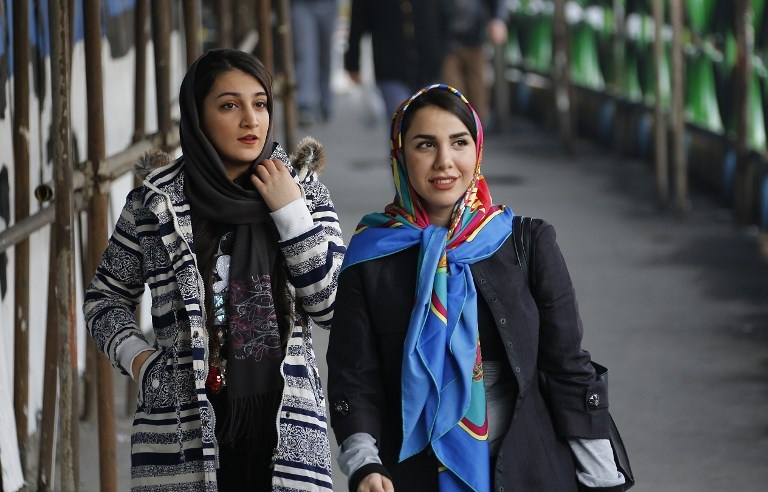
\includegraphics[width=0.3\textwidth]{Orig.jpeg}
        \label{fig:Orig}
    \end{figure}

    \begin{figure}
        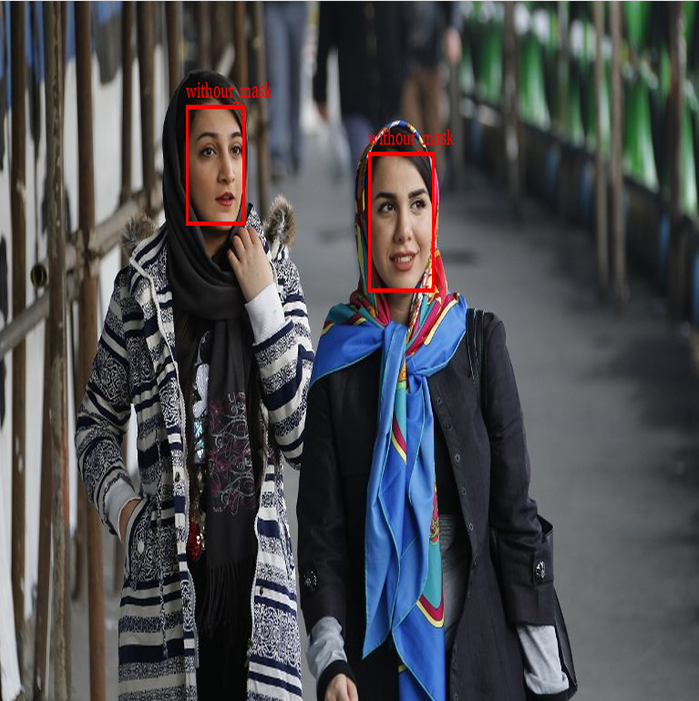
\includegraphics[width=0.3\textwidth]{twoImage-Annotated.png}
        \label{fig:Annotated}
    \end{figure}
\end{frame}

\subsection{Expected Achievements}
\begin{frame}
    \frametitle{Expected Achievements}
    Contents:
    \begin{enumerate}
      \item<1-> Take both datasets and use augmentation to improve pictures.
      \item<2-> Pick two models best suits (CNN) our problem \& search for the best hyper parameters.
      \item<3-> Train two models on datasets and save it for later use
      \begin{itemize}
          \item Fine-tune the human detector model's upper layer
          \item Train mask detector from scratch
      \end{itemize}
      \item<4-> Test it using a GUI or a great integration script (see appendixes section), and run on an unseen test images
    \end{enumerate}
\end{frame}

